\subsubsection{UC36 - Modifica file di configurazione del dizionario dati}\label{UC36}

\begin{figure}[H]
  \centering
  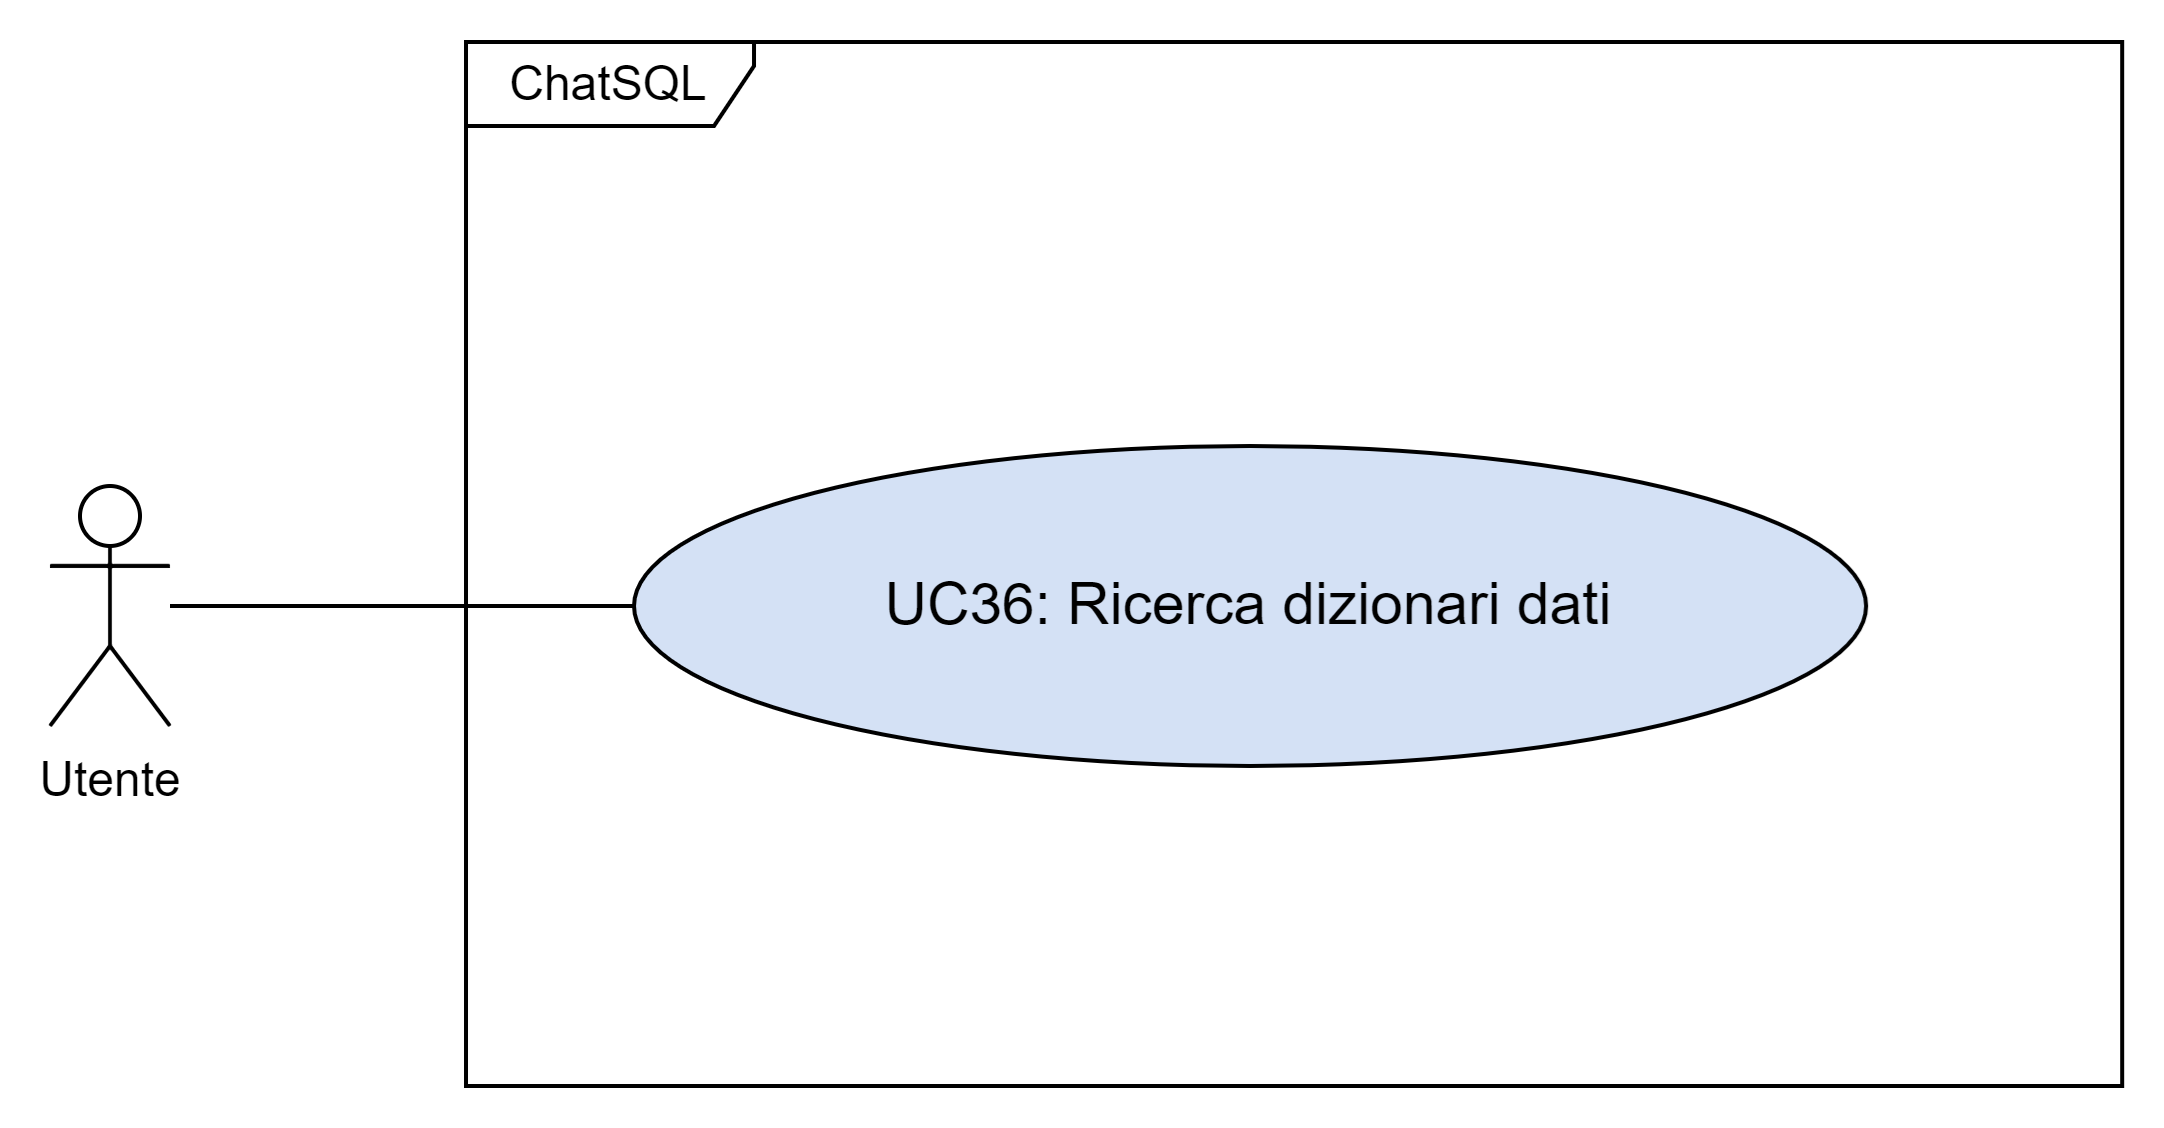
\includegraphics[width=0.90\textwidth]{assets/uc36.png}
  \caption{UC36}
\end{figure}

\paragraph*{Descrizione}
Il Tecnico modifica il file di configurazione del \glossario{dizionario dati}. 

\paragraph*{Attori principali}
Tecnico

\paragraph*{Precondizioni}
\begin{itemize}
  \item Il sistema è attivo e funzionante;
  \item Il Tecnico ha effettuato correttamente l'autenticazione (\hyperref[UC1]{UC1});
  \item Il Tecnico ha visualizzato la lista dei \glossario{dizionari dati} (\hyperref[UC9]{UC9});
  \item Il Tecnico ha scelto il dizionario da modificare (\hyperref[UC9.1]{UC9.1}).
\end{itemize}

\paragraph*{Postcondizioni}
\begin{itemize}
  \item Il file di configurazione del \glossario{dizionario dati} è stato sostituito correttamente.
\end{itemize}

\paragraph*{Trigger}
Il Tecnico vuole modificare il file di configurazione di un \glossario{dizionario dati}.

\paragraph*{Scenario principale}
\begin{enumerate}
  \item Il Tecnico avvia la procedura di modifica del \glossario{dizionario dati};
  \item Il Tecnico inserisce un nuovo file;
  \item Il Tecnico richiede il salvataggio del file;
  \item Il sistema sovrascrive il file precedentemente caricato.
\end{enumerate}

\paragraph*{Scenario alternativo}
\begin{enumerate}
  \item Il sistema riscontra un problema nella validazione del file (\hyperref[UC19]{UC19});
  \item Viene visualizzato un messaggio con i dettagli dell'errore.
\end{enumerate}

\paragraph*{Inclusioni}
\begin{itemize}
  \item Caricamento \glossario{dizionario dati} (\hyperref[UC15]{UC15});
\end{itemize}

\paragraph*{Estensioni}
\begin{itemize}
  \item Visualizzazione errore validazione file (\hyperref[UC19]{UC19}).
\end{itemize}